\documentclass{article}
\usepackage{xcolor}
\usepackage[preprint]{corl_2026}
\usepackage{graphicx,booktabs,amsmath,microtype,longtable,array,placeins,etoolbox}
\usepackage[T1]{fontenc}
\graphicspath{{figures/}}
\definecolor{mover}{HTML}{147D92}
\definecolor{reference}{HTML}{C46635}
\title{Distilling Instructions into Weights:\\Closed-Form Edits Fix a Robot Policy's Misreading}
\author{Ali-Adeeb Abbas$^{1,2}$ and Esmaeil Seraj$^{2}$\thanks{$^1$RIVeR Laboratory, Northeastern University, Boston, MA, USA. $^2$General Motors, Mountain View, CA, USA. Correspondence: \texttt{abbas.a@northeastern.edu}.}}
\hypersetup{pdftitle={Distilling Instructions into Weights: Closed-Form Edits Fix a Robot Policy's Misreading},pdfsubject={arXiv preprint},pdfauthor={Ali-Adeeb Abbas, Esmaeil Seraj}}

% Preprint layout: recover unused title space without changing text size or margins.
\makeatletter
\patchcmd{\@maketitle}{\vskip 0.1in}{\vskip 0pt}{}{\PackageError{preprint-layout}{Title top spacing patch failed}{}}
\patchcmd{\@maketitle}{\vskip 0.3in \@minus 0.1in}{\vskip 0.1in}{}{\PackageError{preprint-layout}{Title bottom spacing patch failed}{}}
\patchcmd{\@maketitle}{\bf\rule{\z@}{24\p@}\@author}{\bf\rule{\z@}{12\p@}\@author}{}{\PackageError{preprint-layout}{Author spacing patch failed}{}}
\patchcmd{\@maketitle}{\bf\rule{\z@}{24\p@}\@author}{\bf\rule{\z@}{12\p@}\@author}{}{\PackageError{preprint-layout}{Preprint author spacing patch failed}{}}
\makeatother

\newcommand{\pifive}{$\pi_{0.5}$}
% Expandable input for table bodies generated by scripts/make_figures.py (plain \input breaks before \bottomrule).
\makeatletter
\newcommand{\tabinput}[1]{\@@input #1 }
\makeatother

\begin{document}
\maketitle
\begin{abstract}
Generalist robot policies often fail at one step of a task they can otherwise perform. We show that such a failure can be removed by editing the policy's weights in closed form, without gradients, training data, or a change to the instruction. Told to put the cube then the banana in the bowl, a zero-shot \pifive{} vision-language-action policy releases the cube before reaching the bowl in RoboLab simulation; replaying 21 of these decisions under rewordings shows that it binds ``in the bowl'' to the wrong object. Closed-form instruction distillation copies an explicit rewording's per-layer residual changes into the language model's MLP weights. On 128 held-out seeds, success rises from 27 to 106 episodes, with 81 fixed and 2 broken (exact McNemar $p=7\times10^{-22}$), whereas an update of the same size in random directions leaves success unchanged. A variant restricted to image tokens, with 0.16\% of the parameter count as low-rank factors, does as well, and the edit lifts two other tasks on held-out seeds without detectable harm on the remaining 13. Across 16 tasks and two editors, edits aimed at perception, a missing grasp, contact physics, or the gripper threshold did not help, and reruns with unchanged weights flipped roughly a third of paired outcomes. Editors should distil a known-good input rather than try to create a missing skill; evaluations should pair seeds, rerun the unedited policy, and confirm gains on held-out seeds.
\end{abstract}
\keywords{Weight Editing, Vision--Language--Action Models, Robot Evaluation}

\setlength{\parskip}{2.5pt}
\setlength{\intextsep}{8pt plus 2pt minus 2pt}
\setlength{\textfloatsep}{12pt plus 2pt minus 2pt}
\section{Introduction}
Generalist vision-language-action (VLA) policies map camera images and an instruction to robot actions, and they often fail at a single step of a task whose skills they already have~\citep{pi2025pi05}; the usual remedy is more demonstrations and fine-tuning. Weight-space programming proposes another: a language model reads a network's weights and activations, locates the computation that goes wrong, and patches the weights directly, without gradients~\citep{takehi2026sparks}. We show that such a patch can fix a generalist robot policy when the failure is a misreading of the instruction, and we map the failures it did not fix.

\begin{figure}[!t]
\centering
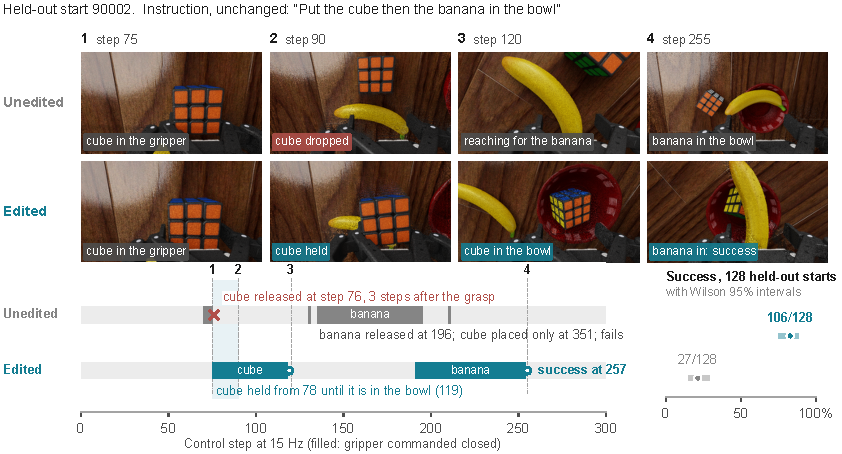
\includegraphics[width=\linewidth]{fig1_teaser.pdf}
\caption{One held-out start, unedited and edited. Top: wrist-camera inputs at four matched control steps. Bottom: commanded gripper (filled where closed) and logged events; with the instruction unchanged, the edit removes the release three steps after the grasp. The explicit rewording ``Put the cube in the bowl then put the banana in the bowl'' was used only to build the edit. Right: held-out success over 128 starts, with Wilson 95\% intervals.}
\label{fig:teaser}
\end{figure}

Early robot reports are encouraging but hard to compare. Guo and Xie report a \pifive{} task rising from 28/92 to 82/92 held-out episodes with four changed parameters, on checkpoints fine-tuned for each task~\citep{guo2026robotweights,xie2026robotweights}. Gupta et al.\ report direct gains on five of ten \pifive{} tasks and a folding gain from 51\% to 75\% with an update built from a difference between trained models~\citep{gupta2026robotweights}. In our companion study, four sparse GPT-6 Astra edits to a zero-shot \pifive{} stacking policy all failed a preservation gate~\citep{abbas2026wspstudy}. We did not reproduce the external results, and together they leave open which failures gradient-free edits can fix in a policy that was never trained on the task.

We study this question with the DROID version of \pifive{}~\citep{pi2025pi05,khazatsky2024droid} on 16 RoboLab tasks~\citep{yang2026robolab}, comparing every edit with the unedited policy on identical simulator seeds. Told to ``put the cube then the banana in the bowl,'' the policy grasps the cube and lets go before reaching the bowl, yet the same weights succeed under an explicit rewording. Robot policies are known to respond differently to equivalent wordings~\citep{fei2026liberoplus,kim2026liberopara,abbas2026samegoal}; here that sensitivity points to a repair. We introduce \emph{closed-form instruction distillation}, which finds such a failure by replaying recorded decisions under rewordings and then writes the internal effect of the working wording into the weights with a multi-key closed-form update~\citep{meng2023memit}. On a held-out start, the edited policy keeps hold of the cube that the unedited policy drops three control steps after grasping it (Fig.~\ref{fig:teaser}).

Our contributions are fourfold. (i) Closed-form instruction distillation, a gradient-free procedure that diagnoses a language-binding failure with instruction-swap replays and copies a known-good instruction's per-layer residual changes into the VLM's MLP weights; to our knowledge it is the first edit that distils an instruction rewording into a robot policy in closed form, and with the instruction unchanged it raises held-out success from 27/128 to 106/128. (ii) Evidence that the edit is specific, can be small, and transfers: an update of the same size in random directions does nothing, a 0.16\% low-rank variant on image tokens matches it on held-out seeds, it lifts two other tasks without detectable harm on the remaining 13, and ablations place the fix in the image tokens. (iii) A map of what such edits did not fix, with two editors and a same-protocol comparison, across perception, missing competence, contact physics, and gripper commitment. (iv) A measurement of the noise floor of paired closed-loop evaluation, where unchanged weights flip roughly a third of paired outcomes, with the smallest detectable effects and the released protocol, code, and paired-episode data.

\section{Closed-Form Instruction Distillation}
\label{sec:method}
Closed-form instruction distillation turns an instruction that works into weights that work: it replays recorded failure decisions under rewordings, identifies a known-good instruction, distils it into the weights in closed form, checks the edit offline, and confirms it in closed loop on practice and then held-out seeds, using only weights, recorded inputs, and activations.

\pifive{} combines an 18-layer PaliGemma vision-language model (VLM) with an 18-layer Gemma action expert~\citep{pi2025pi05,beyer2024paligemma}. The VLM processes image tokens from two cameras with the instruction and robot-state tokens under bidirectional attention, so image tokens can attend to the instruction; the action expert attends to the VLM's keys and values and produces 15-step action chunks, including a gripper command, by flow matching~\citep{black2024pi0}.

The cube-then-banana task illustrates the diagnosis. Under the original instruction the unedited policy succeeds in 9 of 64 episodes. It goes for the cube first in 63 of 64, grasps it, lifts it a few centimetres, and lets go well short of the bowl; we call this a \emph{premature release}. When the cube does reach the bowl first, the episode usually succeeds (about 7 times in 9), so the skill is present. We replayed 21 recorded premature-release decisions with images, robot state, and flow-matching noise fixed, changing only the instruction (Fig.~\ref{fig:construction}a). Renaming the cube leaves all 21 releases, whereas moving ``in the bowl'' next to the cube leaves one to three, and in one VLM attention head the destination words attend far more to the adjacent noun than to the first (Appendix~\ref{app:construction}). We read this as a binding error: holding the cube, the policy treats the banana as the object that belongs in the bowl. The explicit wording is a \emph{known-good instruction}: with unchanged weights it succeeds in 22 of 32 closed-loop episodes against 3 of 32 for the original on the same seeds (20 fixed, 1 broken).

\begin{figure}[!t]
\centering
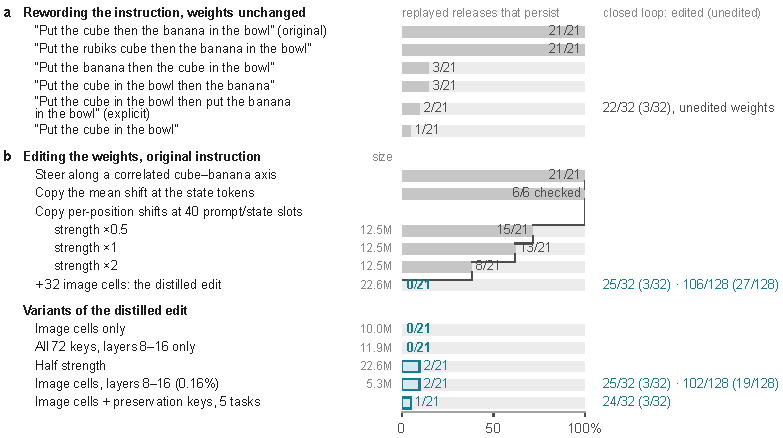
\includegraphics[width=\linewidth]{fig2_construction.pdf}
\caption{What it takes to fix the decision. Bars give the share of 21 recorded premature-release decisions that still release when replayed offline with images, robot state, and noise fixed: (a) under rewordings, (b) under weight edits in the order they were built, then under variants of the distilled edit. Size counts low-rank factors; closed-loop results are edited (unedited) successes on practice $\cdot$ held-out seeds.}
\label{fig:construction}
\end{figure}

Distillation makes the network process the original instruction as it processes the known-good one. At each VLM layer $\ell=0,\dots,16$ we form 72 keys, the rows of $K_\ell$: the mean input to the layer's MLP down-projection under the original instruction at 40 positions shared by both prompts (the beginning-of-sequence, ``Task:'', and robot-state tokens) and at 32 image cells (16 per camera), averaged over 6 recorded premature-release decisions. The matching rows of $V_\ell$ hold the layer's residual increment at that position under the explicit instruction minus that under the original. With activations as row vectors, we apply the regularized minimum-norm update that maps each key to its value,
\begin{equation}
\Delta W_\ell = K_\ell^{\top}\left(K_\ell K_\ell^{\top} + \lambda I\right)^{-1} V_\ell,\qquad \lambda = 10^{-3}\,\mathrm{tr}\!\left(K_\ell K_\ell^{\top}\right)/72,
\label{eq:edit}
\end{equation}
so that $K_\ell \Delta W_\ell \approx V_\ell$. Eq.~\eqref{eq:edit} is the multi-key closed form used to rewrite stored associations in language models~\citep{meng2022rome,meng2023memit}, computed once per layer and here aimed at a rewording. Context distillation trains a model to act as if a prompt were present~\citep{snell2022distilling}, whereas Eq.~\eqref{eq:edit} needs no training. The update has rank at most 72 per layer.

Offline, the edit removes all 21 premature releases and leaves unchanged all 9 recorded correct carries and all 19 phase-two decisions, in which the policy fetches the banana after placing the cube; its actions also land closer to the explicit wording's actions than the unedited ones do (4.5 versus 8.1\,cm at the end of the chunk). On the 32 practice seeds, closed-loop success rises from 3/32 to 25/32, with 22 episodes fixed and none broken (exact McNemar $p=4.8\times10^{-7}$), and we froze the edit for held-out evaluation.

\section{Paired Weight-Edit Evaluation}
\label{sec:eval}
We compare each edited policy with the unedited policy from identical simulator starts, using the OpenPI \pifive{} DROID joint-position checkpoint with about 3.35 billion parameters~\citep{openpi2025,pi2025pi05}. It was trained on DROID data~\citep{khazatsky2024droid} and on none of our tasks, so every result is zero-shot. It receives two $224\times224$ camera images and the joint and gripper state, and it outputs 15-step chunks of seven joint commands and a gripper command binarized at 0.5. We run 16 RoboLab tasks in Isaac Sim with 16 parallel environments per evaluation~\citep{yang2026robolab} and count an episode as a success when RoboLab's terminal success flag is set.

A 16-episode survey of the unedited policy on each task sorted its failures into levels (Appendix~\ref{app:survey}): \emph{language binding}, where the wrong object counts as the current target; \emph{perception}, where the arm goes for a similar-looking object; \emph{missing competence}, where no working motion is produced; \emph{contact physics}, where the decisions look right but the grasp slips; and \emph{gripper commitment}, where open and close decisions sit near the threshold. A motor decision that stalls inside a learned skill, where others report gains~\citep{guo2026robotweights}, did not occur among our tasks.

Edits came from two frontier models run headless: Claude Opus in this work and GPT-6 Astra in the companion study~\citep{abbas2026wspstudy}. An editor can read and write every weight in a NumPy sandbox, capture activations on the exact inputs of any recorded decision, and roll the policy out. It may not use gradients, optimizers, fine-tuning, or black-box search; every edit is a closed-form computation from weights and activations, with its hypothesis written before evaluation, and the instruction text is fixed. Some edits, including the distilled one, were built by the operator session, also Claude Opus, under the same rules; the companion protocol was narrower, with typed operations on at most 128 rows in two action-expert layers (Appendix~\ref{app:other}).

A simulator slot fixes the random seeds and scene of one episode, and every comparison runs both policies on the same slots; these are our \emph{paired seeds}. Each pair has one of four outcomes: both succeed, both fail, \emph{fixed} (only the edited policy succeeds), or \emph{broke} (only the unedited policy succeeds). Edits are developed on \emph{practice seeds}. An edit that passes practice is frozen and scored by the operator on \emph{held-out seeds} never used during editing, with the two policies alternating run order between the halves of the slots. We report paired differences with 95\% bootstrap intervals over the four outcome types (20,000 draws), exact McNemar tests on the fixed and broke pairs~\citep{mcnemar1947note}, and Wilson intervals for single rates~\citep{wilson1927probable}. Because paired seeds do not make episodes identical, we also rerun unedited and identically edited policies as noise controls.

\section{Results}
\label{sec:results}
Closed-form instruction distillation fixes the misreading on seeds never used during editing. On 128 held-out seeds, success rises from 27/128 (21.1\%) to 106/128 (82.8\%), with 81 episodes fixed and 2 broken (+61.7 percentage points, 95\% interval 52.3--70.3; exact McNemar $p=7.2\times10^{-22}$; Fig.~\ref{fig:outcomes}). The Wilson intervals do not overlap, the gain holds in both halves of the alternating run order (Appendix~\ref{app:repro}), and successful episodes finish sooner (300 rather than 412 steps on average). In the event logs, the unedited policy drops the cube during transport, outside the bowl, in 75 of the 81 fixed starts; the edited policy does so in 15 of them and recovers.

The fix comes from the edit's directions, not its size. On the first 64 of these seeds, an update with the same layers, rank, and singular values but random directions scored 9/64, like the unedited policy (13/64 and 9/64 in two runs; exact $p=0.45$ against the first), while the distilled edit scored 50/64 (Appendix~\ref{app:construction}).

\begin{figure}[!t]
\centering
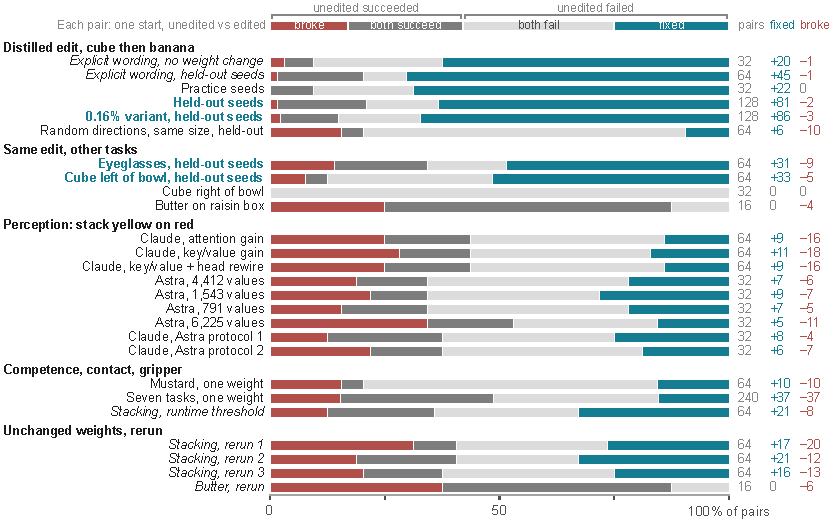
\includegraphics[width=\linewidth]{fig3_outcomes.pdf}
\caption{Paired outcomes. Each bar splits a comparison's paired starts into the four outcome types named in the key; at right, the number of pairs and of fixed and broke pairs. Held-out comparisons are in bold teal; italic rows change no weights. On its own task the distilled edit flips pairs almost only one way; failed edits and unchanged-weight reruns flip many both ways (all comparisons: Appendix~\ref{app:comparisons}).}
\label{fig:outcomes}
\end{figure}

The edit can be made small without losing the effect. Restricting the keys to the 32 image cells in layers 8--16 gives an update of rank at most 32 per layer, with 5.3 million parameters as low-rank factors, or 0.16\% of the parameter count. On the same held-out seeds this variant scores 102/128 against 19/128 (86 fixed, 3 broken; exact $p=3.8\times10^{-22}$), matching the full edit; the unedited policy's 19/128 here and 27/128 in the first run on identical seeds is itself run-to-run variation.

The same edit transfers to two other tasks and harms none detectably. Its keys sit at positions every task has, so we ran it unchanged on all 15 other surveyed tasks (Appendix~\ref{app:sidefx}). On held-out seeds, picking up the eyeglasses rises from 22/64 to 44/64 (31 fixed, 9 broken; +34.4 points, 95\% interval 17.2--51.6; $p=6.8\times10^{-4}$), and putting the cube left of the bowl rises from 8/64 to 36/64 (33 fixed, 5 broken; +43.8 points, 28.1--59.4; $p=4.3\times10^{-6}$). Putting the cube right of the bowl stays at 0/32, so the edit is not a general switch for spatial language. No difference on the remaining 13 tasks is significant (all exact $p\geq0.12$). The largest apparent loss, butter on the raisin box at 10/16 against 14/16, is smaller than the unedited policy's own drop to 8/16 when rerun on the same seeds.

Edits at the other failure levels did not help (Fig.~\ref{fig:outcomes}). In perception, the unedited policy stacks the yellow block on the red block in 28 of 64 practice episodes, and the arm goes first for a nearby Rubik's cube with a yellow face in 48 of 63. The VLM separates the two objects ($d'\approx10$--$20$), but the action expert barely uses the distinction ($d'\approx2$--$3$, against a null of about 1.7). Three Claude edits that amplified this signal through attention or key and value weights each scored 21/64 ($-10.9$ points; 95\% interval $-26.6$ to $+4.7$ for the first) and also suppressed a useful habit of backing away from the cube after touching it. Four GPT-6 Astra edits of 791--6,225 values stayed within noise, and none passed the companion study's gate. A fresh Claude Opus editor under that study's exact protocol independently diagnosed the same lookalike confusion; its two proposals scored 16/32 and 11/32 against 12/32, neither passed the gate, and it submitted the unedited policy (Appendix~\ref{app:other}).

The other levels gave the same answer. The flat green box is never picked up (0/64) because its long side exceeds the gripper opening at the default wrist angle; the best of ten edits raised the share of episodes reaching a graspable wrist angle from 9/16 to 16/16 but produced no success. The mustard bottle slips from a cap grasp mid-carry, and no recorded decision variable predicted which grasps would hold ($|\rho|\leq0.26$); two neuron-flip edits were stopped offline. Built into the network as one bias weight, the companion study's lower gripper threshold~\citep{abbas2026wspstudy} scored 117/240 against 117/240 across seven tasks, with 37 episodes fixed and 37 broken.

\begin{figure}[!t]
\centering
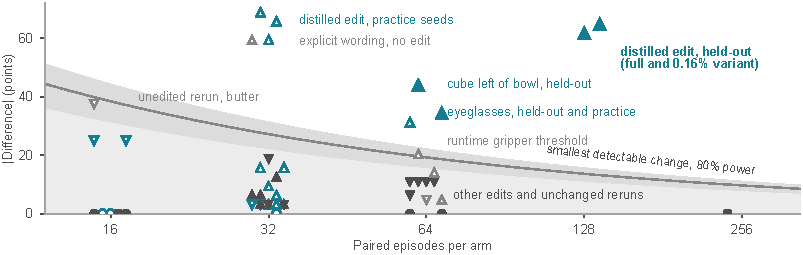
\includegraphics[width=\linewidth]{fig4_detectability.pdf}
\caption{Which differences a paired comparison can detect. Markers place each comparison by its paired episodes and the size of its difference, pointing up when the edit did better; below the curve a difference is smaller than the change detectable with 80\% power ($\alpha=0.05$, 30\% of pairs discordant; band 20--40\%). Teal: distilled edit (filled: held-out); gray: no weight change; dark: other edits.}
\label{fig:detect}
\end{figure}

Paired seeds still leave large run-to-run variation. The unedited policy scored 14/16 and then 8/16 on the same 16 butter seeds, two runs of one edited policy agreed on only 46 of 64 paired episodes, and a near-neutral one-weight edit changed 70 of 192 paired outcomes on tasks with room to move. With about 30\% of pairs discordant, a single paired comparison with 80\% power at $\alpha=0.05$ detects changes of about 27 points with 32 pairs, 19 with 64, 14 with 128, and 10 with 256 (Fig.~\ref{fig:detect}). A 16-episode screen is therefore a filter, not evidence: the distilled edit clears this bound on held-out seeds, whereas every failed edit and every unchanged-weight rerun falls below it, the butter rerun only just.

\section{Why Some Failures Can Be Edited}
\label{sec:why}
The image tokens carry the fix. Three simpler edits failed offline (Fig.~\ref{fig:construction}b): steering image tokens along a cube-versus-banana axis that tracks the wording flipped none of the 21 releases even at three times the explicit wording's value, so the axis was correlated with the outcome but not causal~\citep{turner2023steering}; copying the mean shift at the state tokens flipped none; and copying per-token shifts at the 40 prompt and state positions left 8 to 15. Adding the 32 image cells removed all 21, and image cells alone suffice, whereas prompt and state positions alone leave 13 (Appendix~\ref{app:construction}). The explicit wording moves the image tokens by only 2--4\% of their norm, yet the action expert places 13--44\% of its attention on them. Because prefix attention is bidirectional, image tokens attend to the instruction; our working hypothesis is that the instruction is read into the image representation that the action expert consults when it decides whether to keep holding.

Distillation re-routes a computation the network already performs; it did not create one that is missing. The success had three ingredients: a skill the policy demonstrably has, a failure traced to one computation, and a known-good internal state to copy. Each failed level lacked one: the flat box lacks the skill, the mustard grasp has no wrong decision to correct, and in perception no edit we found routed the VLM's correct signal to the action without breaking a useful behavior. This agrees with the strongest outside reports, which edited checkpoints already fine-tuned on each task~\citep{guo2026robotweights} or built updates from differences between trained models~\citep{gupta2026robotweights,ilharco2023arithmetic}. It suggests a practical rule: edit when the network can be shown to do the right thing under some input, and train when it cannot.

These conclusions have limits. The full edit is low-rank but not sparse: it changes 13.4\% of the policy's stored values, and the 0.16\% variant still changes about 7\% once applied. Discovery needed a known-good instruction, which turns a prompt fix into a weight fix when the instruction cannot be changed but does not help when no input succeeds. The edit was built by the operator session under the editor rules, not by an autonomous editor. Transfer was not predicted in advance (left of the bowl but not right), so deployment would need broad regression checks. All results come from one zero-shot checkpoint in simulation, with 16 to 128 pairs per comparison and failure levels assigned without an independent rater.

\section{Concluding Remarks}
Closed-form instruction distillation fixed a misread instruction in a zero-shot generalist VLA without gradients or a change to the instruction; a random update of the same size did not, and a 0.16\% low-rank version worked as well. Edits aimed at perception, missing competence, contact physics, and the gripper threshold did not help, which places the method's reach at failures that some known-good input can expose: find an input under which the policy succeeds, distil its internal state, and confirm the gain on paired held-out seeds. Next steps are autonomous editors on the binding task, task-fine-tuned checkpoints, smaller edits, and a physical robot.

\clearpage
\bibliography{refs}
\clearpage
\appendix

\setlength{\parskip}{5.5pt}
\section{Unedited-policy survey and failure levels}
\label{app:survey}
Table~\ref{tab:survey} lists the 16 RoboLab tasks with the unedited policy's success in 16 episodes and its dominant failure classes. Episodes last 450 or 900 control steps at 15\,Hz, depending on the task. Failure classes come from RoboLab events and recorded gripper commands. The ``wrong object first'' class relies on a RoboLab event that the companion study's audit found to over-count~\citep{abbas2026wspstudy}, so those counts are upper bounds. Levels for the five case-study tasks rest on editor diagnoses from kinematics, camera frames, and activation captures; no independent rater checked them.

\begin{table}[htbp]
\centering\small
\caption{Unedited policy, 16 episodes per task. Failure classes are dominant counts among the failed episodes.}
\label{tab:survey}
\begin{tabular}{@{}p{.36\linewidth}rp{.44\linewidth}@{}}
\toprule
Task & Success & Dominant failure classes\\
\midrule
\tabinput{generated/survey_table.tex}
\bottomrule
\end{tabular}
\end{table}

\begin{table}[htbp]
\centering\small
\caption{Failure levels and what weight editing did at each. Counts are edited versus unedited on paired seeds unless stated.}
\label{tab:levels}
\begin{tabular}{@{}>{\raggedright\arraybackslash}p{.16\linewidth}>{\raggedright\arraybackslash}p{.26\linewidth}>{\raggedright\arraybackslash}p{.15\linewidth}>{\raggedright\arraybackslash}p{.32\linewidth}@{}}
\toprule
Level & What goes wrong & Example & Weight editing\\
\midrule
Language binding & The wrong object counts as the current target & Cube then banana & Held-out 106/128 vs 27/128; transfers to eyeglasses and cube left of bowl\\
Perception & Goes for a similar-looking object & Stack yellow on red & 3 Claude edits at $-$10.9 points; 4 Astra and 2 same-protocol Claude proposals, none accepted\\
Missing competence & Never produces a working motion & Pick up flat box & 10 edits change the motion, 0 successes\\
Contact physics & Decisions look right, the grasp slips & Mustard into bin & No decision-level lever; edits stopped offline; one weight 13/64 vs 13/64\\
Gripper commitment & Open and close decisions near the threshold & Seven tasks & One weight, 117/240 vs 117/240\\
Motor decision, skill present & A competent skill stalls at one step & None among our 16 tasks & Not tested; others report gains on task-fine-tuned checkpoints\\
\bottomrule
\end{tabular}
\end{table}

\FloatBarrier
\section{All paired comparisons and the noise floor}
\label{app:comparisons}
Table~\ref{tab:all} lists every closed-loop comparison in \texttt{study/results/opus/comparisons.json}, and Fig.~\ref{fig:outcomes-full} shows the paired outcomes of each. Each difference is edited minus unedited on paired seeds, in percentage points, with a 95\% interval from 20,000 multinomial draws over the four paired outcome types (both succeed, fixed, broken, both fail). The pooled gripper row is resampled within each task. The $p$-values are exact two-sided McNemar tests on the fixed and broken pairs. The companion study's rows use its own runtime and are not pooled with ours. Its unchanged-weight rerun labelled ``extra'' shares the unedited reference of the first rerun, so those two comparisons are correlated. Rows that begin with Astra are GPT-6 Astra edits and rows marked Astra study are the companion study's operator controls; all other edits, including the two under the Astra protocol, are Claude Opus edits.

{\fontsize{8}{9.6}\selectfont
\setlength{\tabcolsep}{2.6pt}
\setlength{\LTcapwidth}{\linewidth}
\begin{longtable}{@{}>{\raggedright\arraybackslash}p{.27\linewidth}rlcll@{}}
\caption{Every paired closed-loop comparison. Values: stored scalar values changed by the edit (--- for none or not recorded). Counts: edited versus unedited successes on the same seeds. Difference in percentage points.}
\label{tab:all}\\
\toprule
Comparison & Values & Counts & Fixed / broke & Difference [95\% CI] & $p$\\
\midrule
\endfirsthead
\toprule
Comparison & Values & Counts & Fixed / broke & Difference [95\% CI] & $p$\\
\midrule
\endhead
\tabinput{generated/comparisons_table.tex}
\bottomrule
\end{longtable}
}

\paragraph{Noise floor.} Unchanged weights do not give unchanged outcomes on paired seeds. The share of paired episodes whose outcome differs is 28\% for two runs of one edited policy, 36\% for a near-neutral one-weight edit on the four tasks with room to move, 38\% for the unedited butter rerun, and 45--58\% for the companion study's unchanged-weight reruns (Fig.~\ref{fig:outcomes-full}). The companion study's audit found different first camera images and actions in paired episodes with equal seeds and robot state, without isolating the cause~\citep{abbas2026wspstudy}; nondeterministic GPU simulation amplified by open-loop action chunks is one candidate. Table~\ref{tab:mde} gives the smallest paired difference a single comparison detects with 80\% power at a two-sided $\alpha=0.05$, using the normal approximation $(z_{0.975}+z_{0.8})\sqrt{q/n}$ with a discordant fraction $q=0.3$. Fig.~\ref{fig:detect} places every observed effect against that bound.

\begin{table}[htbp]
\centering\small
\caption{Smallest detectable paired difference with about 30\% discordant pairs (80\% power, $\alpha=0.05$).}
\label{tab:mde}
\begin{tabular}{@{}rr@{}}
\toprule
Paired episodes per arm & Smallest detectable change\\
\midrule
32 & about 27 points\\
64 & about 19 points\\
128 & about 14 points\\
256 & about 10 points\\
\bottomrule
\end{tabular}
\end{table}

\begin{figure}[p]
\centering
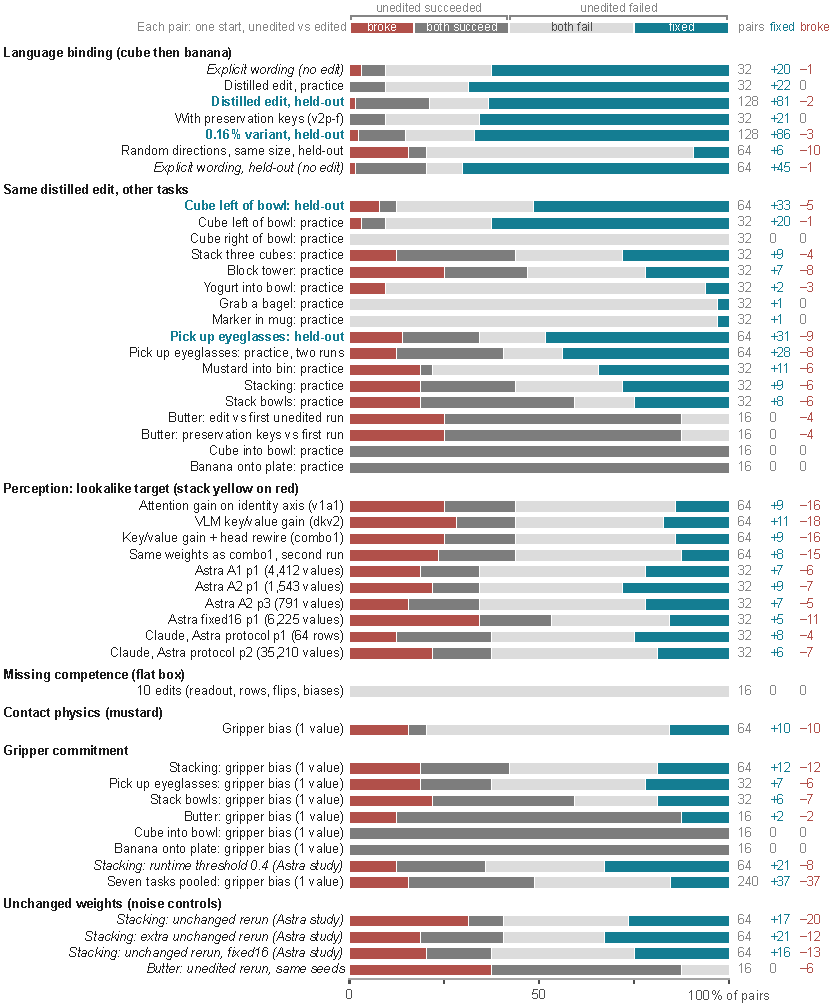
\includegraphics[width=\linewidth]{figA_outcomes_full.pdf}
\caption{Paired outcomes of every comparison in Table~\ref{tab:all}, drawn as in Fig.~\ref{fig:outcomes}. Held-out comparisons are in bold teal. The flat-box row stands for each of the ten edits, all 0/16 against an unedited 0/64.}
\label{fig:outcomes-full}
\end{figure}

\FloatBarrier
\section{Edit construction, failed attempts, and ablations}
\label{app:construction}
\paragraph{Capture and tensors.} The edit uses one activation capture of 6 premature-release decisions, each replayed under 8 instructions, with VLM residuals and MLP activations at every layer. It modifies the MLP down-projections \texttt{language.blocks.00--16.mlp.linear}, each mapping 16,384 hidden features to the 2,048-dimensional residual stream. Keys are mean activations under the original instruction; values are the explicit instruction's per-layer residual increments minus the original's. Each layer receives Eq.~\eqref{eq:edit} with $\lambda=10^{-3}\,\mathrm{tr}(KK^{\top})/n$ for $n$ keys and unit strength. After rounding to bfloat16, the full edit changes 450,468,837 stored values (13.4\%) with rank at most 72 per layer.

\paragraph{Attempts that failed offline.} All of these were stopped by offline replay on recorded decisions, before any rollout (Fig.~\ref{fig:construction}b). Two rank-one pushes along a cube-versus-banana ``target'' axis at the image tokens left 21 of 21 releases. Copying the mean explicit-minus-original shift at the state tokens, rank one per layer, left 6 of 6 releases on a six-decision check. Copying the per-position shift at the 40 prompt and state positions with Eq.~\eqref{eq:edit} left 15, 13, and 8 of 21 releases at strengths 0.5, 1, and 2 (candidates \texttt{v2m-h}, \texttt{v2m-f}, \texttt{v2m-2}), and adding text positions left 13. Adding the 32 image cells gave the submitted edit, with 0 of 21 releases and unchanged carries and phase-two decisions.

\paragraph{Ablations and the 0.16\% variant.} Table~\ref{tab:ablation} lists the offline ablations shown in Fig.~\ref{fig:construction}b, with their layers, keys, and sizes. Applied to the weights, every variant still changes 248--450 million stored values (7--13\%), because each low-rank update is dense in the weight matrix. The smallest variant (image cells, layers 8--16, rank at most 32) changes 248,057,499 values. In closed loop it scores 25/32 against 3/32 on the practice seeds (22 fixed, 0 broken). On held-out seeds 90000--90127 it scores 102/128 against 19/128 (86 fixed, 3 broken; exact $p=3.8\times10^{-22}$), with Wilson intervals of 71.9--85.7\% and 9.7--22.0\%; successful episodes take 333 rather than 396 steps on average.

\paragraph{Random-direction control.} For each of layers 0--16 we recomputed the distilled update in float64 from the same capture (it reproduces the stored edit exactly after bf16 rounding), kept its 72 singular values, and replaced its left and right singular vectors with random orthonormal bases (NumPy \texttt{default\_rng(0)}). The control therefore matches the edit's layers, rank, singular values, and Frobenius norm in every layer; it changes 502,291,925 stored values (15.0\%) against the edit's 450,468,837 (13.4\%). Frozen and fingerprinted like a submission, it was run by the operator on held-out seeds 90000--90063 and scored 9/64, against 13/64 and 9/64 for the unedited policy's two runs on those seeds (6 fixed and 10 broken, exact $p=0.45$; 4 and 4, $p=1$) and 50/64 for the distilled edit (0 fixed and 41 broken relative to it).

\begin{table}[htbp]
\centering\small
\caption{Offline ablations of Eq.~\eqref{eq:edit} on the 21 recorded premature releases; every variant keeps all 9 correct carries and 19 phase-two decisions. Factored size is rank $\times$ (16{,}384 + 2{,}048) $\times$ layers, with its share of the parameter count. Held-out: edited versus unedited successes of 128.}
\label{tab:ablation}
\setlength{\tabcolsep}{5pt}
\begin{tabular}{@{}llrrrr@{}}
\toprule
Variant & Layers & Keys per layer & Factored size & Releases (of 21) & Held-out\\
\midrule
Full edit & 0--16 & 72 & 22.6M (0.67\%) & 0 & 106 vs 27\\
Image cells only & 0--16 & 32 & 10.0M (0.30\%) & 0 & ---\\
Layers 8--16 only & 8--16 & 72 & 11.9M (0.36\%) & 0 & ---\\
Half strength & 0--16 & 72 & 22.6M (0.67\%) & 2 & ---\\
Image cells, layers 8--16 & 8--16 & 32 & 5.3M (0.16\%) & 2 & 102 vs 19\\
Prompt and state positions only & 0--16 & 40 & 12.5M (0.37\%) & 13 & ---\\
\bottomrule
\end{tabular}
\end{table}

\paragraph{Diagnosis details.} The destination words' attention to the adjacent noun versus the first noun is 0.69 versus 0.02 in VLM layer 1, head 1. The explicit wording changes the image tokens by 2--4\% of their norm, while the action expert places 13--44\% of its attention on image tokens and 33--58\% on the instruction and state tokens. On recorded decisions, the edited policy's actions land 4.5\,cm from the explicit wording's actions at the end of the chunk, against 8.1\,cm for the unedited policy.

\FloatBarrier
\section{Edits at the other failure levels}
\label{app:other}
\paragraph{Perception: stack yellow on red.} The Claude cohort built three edits that amplify the VLM's yellow-versus-cube distinction in the action pathway: an attention gain on an identity axis (30.4 million values), a VLM key and value gain (12.0 million), and that gain combined with an attention-head rewire (12.2 million). Each scored 21/64 against 28/64; a second run of the combined edit with identical weights scored 21/64 again, with different fixed and broken episodes (8 and 15 instead of 9 and 16). Several further stacking candidates were built but never evaluated in closed loop. The companion study's four Astra edits changed 4,412, 1,543, 791, and 6,225 values in selected action-expert MLP rows and scored 12/32, 13/32, and 13/32 against 11/32, and 11/32 against 17/32 in a separate runtime~\citep{abbas2026wspstudy}.

\paragraph{Claude Opus under the companion protocol.} We gave a fresh Claude Opus editor the companion study's brief for the stacking task. It received the same 32 development episodes, at most three candidate evaluations on those slots, 96 activation items, and 7,200 seconds. Edits were limited to the action expert's MLP output rows, at most 128 rows across two layers, through typed operations (row scaling, adding a direction to rows, projecting a direction out of rows), with no fitted regression or search. The fixed gate accepts a candidate only with strictly more successes than the unedited 12/32 and at most two newly broken pairs. The editor found that the main failure is confusion with yellow-looking distractors, decided by noise in the first action chunks: in 13 of 32 unedited episodes the first grasp was the Rubik's cube, and 3 of those 13 succeeded against 9 of 17 when the yellow block came first. Its first proposal added a direction to 64 rows of the last action-expert layer and scored 16/32 against 12/32 with 8 fixed and 4 broken, so the gate rejected it; its own check found that the predicted shift of the first chunk toward the yellow block did not occur beyond run-to-run variation. A half-strength second proposal scored 11/32 (6 fixed, 7 broken). The editor declined a third proposal as ``another dose of a falsified lever, effectively a lottery draw,'' and submitted the unedited policy after 2 of 3 evaluations, 64 of 96 activation items, and about 7,000 of 7,200 seconds, for about \$20 of API use.

\paragraph{Missing competence: pick up the flat box.} The unedited policy is 0/64. The box's long side is wider than the gripper opening, so at the default wrist angle the fingers land on top of it; when the wrist does rotate, the close command flip-flops. Ten edits were tried: readout surgery, neuron flips, a ``stay closed'' latch, and wrist and gripper biases. Nine scored 0/16 and one 0/32. The best raised the share of episodes reaching a graspable wrist angle from 9/16 to 16/16 in closed loop, without a success.

\paragraph{Contact physics: put the mustard in the bin.} The unedited policy succeeds in 16 of 96 episodes. It grabs the bottle by its narrow cap and keeps the gripper commanded closed, and in most episodes the bottle slips mid-carry (Fig.~\ref{fig:mustard}). Close height, wrist angle, timing, and carry speed did not predict which grasps hold ($|\rho|\leq0.26$). Two neuron-flip edits in the style of Gupta et al.~\citep{gupta2026robotweights}, built from 192 recorded grasps and changing 131,072 and 1,048,576 values, either left the actions nearly unchanged (0.0005\,rad mean joint change and 0 of 96 flipped decisions) or pushed them the wrong way, and both were stopped offline. The one-weight gripper edit scored 13/64 against 13/64.

\begin{figure}[htbp]
\centering
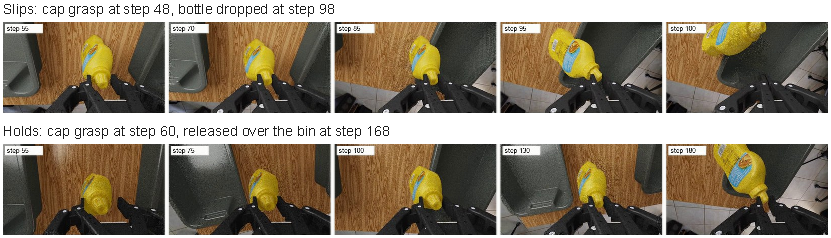
\includegraphics[width=\linewidth]{figA_mustard.pdf}
\caption{Wrist camera, mustard into bin, unedited policy. Both rows grip the cap; the top grasp slips and the bottom one holds. No recorded decision variable separated them.}
\label{fig:mustard}
\end{figure}

\paragraph{Gripper commitment.} The companion study's largest effect was a runtime change that binarizes the gripper at 0.4 instead of 0.5: 36/64 against 23/64 on stacking, while its own unchanged-weight repeat also moved from 26 to 35. We built the same shift into the network as one scalar, the gripper output bias. On fixed recorded inputs it raised the mean gripper command by 0.109 and the number of closed rows from 674 to 781 of 1,440. In closed loop it was exactly neutral (Table~\ref{tab:gripper}).

\begin{table}[htbp]
\centering\small
\caption{One-weight gripper edit, edited versus unedited on paired seeds.}
\label{tab:gripper}
\begin{tabular}{@{}lrrrr@{}}
\toprule
Task & Pairs & Unedited & Edited & Fixed / broke\\
\midrule
\tabinput{generated/gripper_table.tex}
\bottomrule
\end{tabular}
\end{table}

\FloatBarrier
\section{Side effects and transfer}
\label{app:sidefx}
\paragraph{Transfer map.} Table~\ref{tab:transfer} lists the distilled edit on all 15 other surveyed tasks. The first seven other tasks were compared with an earlier unedited run on the same slots; the transfer map of eight more tasks ran the unedited and edited policies back to back on the same 32 slots. Held-out runs used slots 90000--90063, with the run order alternating by half. Eyeglasses failures are often grasps that are never lifted. We hypothesize that the edit strengthens a generic signal that the held object is the one to carry, so the policy keeps hold and persists; successful held-out eyeglasses episodes take longer with the edit (224 versus 158 steps on average). The left-of-bowl gain without a right-of-bowl gain shows that the edit is not a general switch for spatial language; our working hypothesis is that it strengthens how the network ties a destination phrase to the carried object, and that something else fails first in the right-of-bowl task. Neither hypothesis has been tested.

\begin{table}[htbp]
\centering\fontsize{8}{9.6}\selectfont
\setlength{\tabcolsep}{3.2pt}
\caption{The distilled edit on the other surveyed tasks, edited versus unedited on paired seeds. Difference in percentage points with its paired 95\% bootstrap interval; $p$ from the exact McNemar test. The last row is the unedited butter rerun.}
\label{tab:transfer}
\begin{tabular}{@{}lrrrcll@{}}
\toprule
Task & Pairs & Unedited & Edited & Fixed / broke & Difference [95\% CI] & $p$\\
\midrule
\tabinput{generated/transfer_table.tex}
\bottomrule
\end{tabular}
\end{table}

\paragraph{The butter identity rerun.} Butter on the raisin box first looked like a loss, 10/16 against 14/16 with 0 fixed and 4 broken. Rerun on the same 16 seeds with the same weights, the unedited policy itself scored 8/16 (0 fixed and 6 broken against its first run; exact $p=0.031$). The edit's paired bootstrap interval against the first run excludes zero ($-50.0$ to $-6.2$ points; exact $p=0.12$), but so does the unedited rerun's interval against the same run, with a larger drop ($-62.5$ to $-12.5$). The comparison therefore cannot separate an edit effect from the policy's own run-to-run variation.

\paragraph{Preservation keys.} We rebuilt the edit with image-cell keys plus 160 preservation keys (32 image cells from each of five other tasks, each mapped to a zero change) in layers 0--16. Offline it left 1 of 21 releases. In closed loop it kept the fix, 24/32 against 3/32 with 21 fixed and none broken, and scored the same on butter (10/16). There was no real side effect for it to remove.

\paragraph{Evaluation lanes.} The distilled-edit runs used two evaluation lanes. Across those runs, success was 249/448 on one lane and 199/368 on the other, with no lane effect.

\FloatBarrier
\section{Reproducibility}
\label{app:repro}
\paragraph{Code and data.} The paired outcomes behind every comparison in this paper are in the repository \url{https://github.com/adeeb10abbas/weightsmith}. The paired comparisons are in \texttt{study/results/opus/comparisons.json}, and the four held-out runs, with per-slot outcomes, Wilson intervals, and exact McNemar tests, are in \texttt{study/results/opus/heldout/}. The evidence record \texttt{study/results/opus/EVIDENCE.md} lists every proposal, budget, and cost; the edit scripts are in \texttt{study/results/opus/ctb/}, and the brief and final report of the same-protocol run are in \texttt{study/results/opus/}. The command \texttt{python3 paper/scripts/make\_figures.py} regenerates every figure and generated table of this paper from these files.

\paragraph{Held-out protocol.} The operator scored frozen edits with \texttt{weightsmith/heldout.py} on slots 90000--90127 (cube then banana) and 90000--90063 (transfer tasks). The first half of the slots ran the unedited policy first and the second half the edited policy first. Editors never saw held-out slots. On cube then banana, the Wilson 95\% intervals are 75.3--88.4\% for the edited and 14.9--29.0\% for the unedited policy. The random-direction control ran later with \texttt{study/results/opus/controls/ctl\_run.py} on slots 90000--90063 and is paired with the unedited runs recorded there. Table~\ref{tab:halves} splits each held-out run by run order; every gain appears in both halves. The RoboLab event logs of the cube-then-banana run are summarized per slot in \texttt{paper/figures/src/heldout\_v2mif\_events.json}, which gives the cube-drop counts in Section~\ref{sec:results}. Fig.~\ref{fig:teaser} shows the lowest-numbered fixed start whose unedited run dropped the cube before touching the banana, start 90002; its frames, gripper commands, and events come from the recorded episodes (\texttt{paper/scripts/build\_teaser\_data.py}).

\begin{table}[htbp]
\centering\small
\caption{Held-out runs split by run order, from the per-slot outcomes. Counts are successes out of the slots in each half.}
\label{tab:halves}
\begin{tabular}{@{}llllll@{}}
\toprule
Run & Slots & Order & Unedited & Edited & Fixed / broke\\
\midrule
\tabinput{generated/heldout_halves_table.tex}
\bottomrule
\end{tabular}
\end{table}

\paragraph{Runtime and editors.} Evaluations used RoboLab on Isaac Sim with the performance preset and 16 environments per evaluation; the original cohort ran on one RTX 3090. The runtime code is identical to commit \texttt{f503fb3} of the repository, and the checkpoint is pinned by \texttt{third\_party/pi05\_droid\_jointpos.sha256}. Claude Opus editors ran headless through Claude Code, with tool access limited to the editing command and file operations, all 730 weight tensors editable, and budgets of 1,200 (stacking) or 800 (flat box) practice episodes and 6,000 activation items. Practice slots were 20000--20063 for stacking and 60000--60063 for the flat box and mustard; the cube-then-banana practice runs used slots 20000--20031. Raw episodes, activation captures, and candidate weights remain on the GPU host and are not in the repository.

\paragraph{Cost.} Recorded editor API spend for the Claude Opus cohort was about \$799: \$632 for the stacking editor, \$94 for the first project, and \$73 for the flat-box editors. The same-protocol run cost about \$20. Operator sessions and GPU time were not metered.

\end{document}
